\section{Controls, status and camera views}
\label{sec:controls}
\begin{figure}[H]\centering
\begin{minipage}{0.54\linewidth}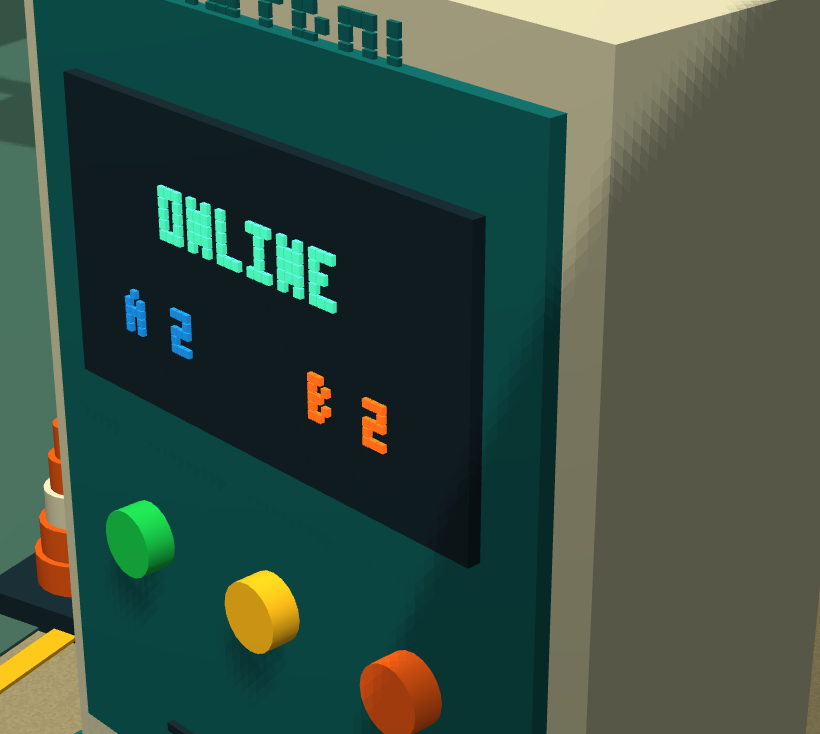
\includegraphics[width=\linewidth,height=55mm,keepaspectratio]{assets/cabinet_crop.png}\par\small\textbf{Cabinet at 24 s:} ONLINE, A = 2, B = 2. The modeled buttons are decorative.\end{minipage}\hfill
\begin{minipage}{0.42\linewidth}\small
\textbf{System status}\par
The cabinet shows running/paused and two collection counts. The tower shows the current operating stage. Brightness is emission: active 1.00, inactive 0.03.
\end{minipage}
\caption{Close-up of the actual status display and its geometric lettering.}
\end{figure}
\begin{figure}[H]\centering
\begin{minipage}{0.31\linewidth}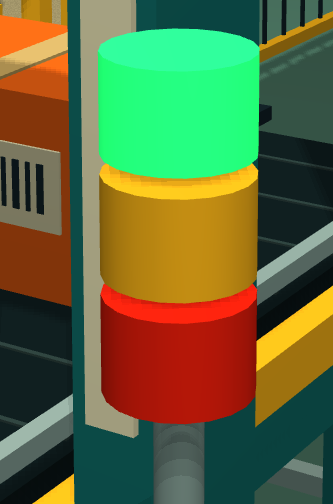
\includegraphics[width=\linewidth,height=34mm,keepaspectratio]{assets/tower_run_crop.png}\par\small\textbf{Green: running.}\end{minipage}\hfill
\begin{minipage}{0.31\linewidth}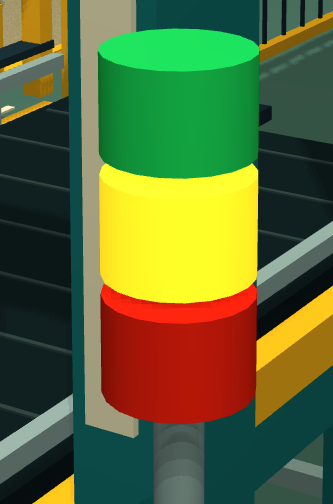
\includegraphics[width=\linewidth,height=34mm,keepaspectratio]{assets/tower_scan_crop.png}\par\small\textbf{Yellow: scanning.}\end{minipage}\hfill
\begin{minipage}{0.31\linewidth}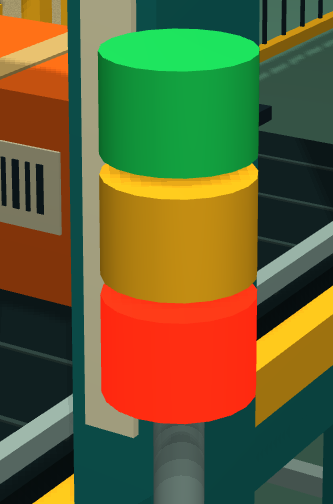
\includegraphics[width=\linewidth,height=34mm,keepaspectratio]{assets/tower_pause_crop.png}\par\small\textbf{Red: paused.}\end{minipage}
\caption{Same tower view, cropped equally. Run/pause are at 24 s; scanning is at 6.70 s.}
\end{figure}
\par{\small\begin{tabularx}{\textwidth}{@{}L{35mm}Y@{}}\toprule
\textbf{Input} & \textbf{Action}\\\midrule
\code{Space}; \code{+/-} & Pause/resume; change conveyor speed. Fan and camera continue during pause.\\
\code{G}; \code{L}; \code{P} & Request gate test; toggle point lights; switch Phong/Gouraud.\\
\code{R} & Reset parcels, counts, timers and angles; speed 1.55; resume. Camera/shading/light choice stay unchanged.\\
\code{1 / 2 / 3} & Overview / top / side camera presets.\\
\code{W A S D}; \code{Q/E} & Move camera forward/left/back/right; down/up at 8 units/s.\\
Mouse; wheel & Look around; zoom between $25^\circ$ and $70^\circ$ field of view.\\
\code{Tab}; click; \code{F11}; \code{Esc} & Release/recapture mouse; display mode; exit.\\\bottomrule
\end{tabularx}}\par
\subsection{Camera model and overhead view}
\begin{shot}{assets/top_layout.png}{Overhead factory view at 24 s. The upper and lower conveyors, scanner and branching exits define the sorting path.}
\callout{0.19,0.50}{0.18,0.85}{Entry conveyor}
\callout{0.54,0.51}{0.79,0.50}{Scanner}
\callout{0.68,0.50}{0.19,0.35}{Two-way sorter}
\end{shot}
\textbf{Camera implementation:} \code{glm::lookAt} constructs the view matrix. Perspective uses a $50^\circ$ default field of view, aspect ratio $W/H$, near plane 0.1 and far plane 100. Vertex position is $PVMp$. The top preset also uses perspective projection. Walls near the camera are omitted; at camera height 20 or above, beam and lamp meshes are omitted to reveal the conveyor layout. These rules also affect the shadow pass.
\source{\code{Camera.cpp}; \code{main.cpp}: callbacks and camera projection; \code{FactoryScene.cpp}: cabinet, tower and cutaway.}
